%%%%%%%%%%%%%%%%%%%%%%%%%%%%%%%%%%%%%%%%%
% Stylish Article
% LaTeX Template
% Version 2.1 (1/10/15)
%
% This template has been downloaded from:
% http://www.LaTeXTemplates.com
%
% Original author:
% Mathias Legrand (legrand.mathias@gmail.com) 
% With extensive modifications by:
% Vel (vel@latextemplates.com)
%
% License:
% CC BY-NC-SA 3.0 (http://creativecommons.org/licenses/by-nc-sa/3.0/)
%
%%%%%%%%%%%%%%%%%%%%%%%%%%%%%%%%%%%%%%%%%

%----------------------------------------------------------------------------------------
%	PACKAGES AND OTHER DOCUMENT CONFIGURATIONS
%----------------------------------------------------------------------------------------

\documentclass[fleqn,10pt]{SelfArx} % Document font size and equations flushed left
\usepackage[T1]{fontenc}
\usepackage[utf8]{inputenc}
%\usepackage[english]{babel}
\usepackage[italian]{babel} % Specify a different language here - english by default

%\usepackage{lipsum} % Required to insert dummy text. To be removed otherwise
\usepackage{graphicx}
\usepackage{amsmath}
\usepackage{amssymb}
\usepackage[skip=3pt, labelfont=bf, width=80mm]{caption}
\captionsetup[figure]{font=small,labelfont=small}

\usepackage{comment}
\usepackage{mathtools}

%\usepackage{titlesec}

%\titlespacing*{\section}{0pt}{ plus 1ex minus .2ex}{4.3ex plus .2ex}
%\titlespacing*{\subsection}{0pt}{3ex plus 0.5ex minus .2ex}{1ex plus .2ex}
%\titlespacing*{\subsubsection}{0pt}{std}{1ex plus .2ex}

%----------------------------------------------------------------------------------------
%	COLUMNS
%----------------------------------------------------------------------------------------

\setlength{\columnsep}{0.55cm} % Distance between the two columns of text
\setlength{\fboxrule}{0.75pt} % Width of the border around the abstract

%----------------------------------------------------------------------------------------
%	COLORS
%----------------------------------------------------------------------------------------

%\definecolor{color1}{RGB}{0,0,90} % Color of the article title and sections
\definecolor{color1}{RGB}{128,0,0}
\definecolor{color2}{RGB}{0,20,20} % Color of the boxes behind the abstract and headings

\renewcommand{\topfraction}{0.85}
\renewcommand{\bottomfraction}{0.85}
%\renewcommand{\textfraction}{0.15}
\renewcommand{\floatpagefraction}{0.85}
\renewcommand{\textfraction}{0.15}
%----------------------------------------------------------------------------------------
%	HYPERLINKS
%----------------------------------------------------------------------------------------

\usepackage{hyperref} % Required for hyperlinks
\hypersetup{hidelinks,colorlinks,breaklinks=true,urlcolor=color2,citecolor=color1,linkcolor=color1,bookmarksopen=false,pdftitle={Title},pdfauthor={Author}}

%----------------------------------------------------------------------------------------
%	ARTICLE INFORMATION
%----------------------------------------------------------------------------------------

\JournalInfo{ $\ $ } % Journal information

%\JournalInfo{FIXME }
\Archive{ } % Additional notes (e.g. copyright, DOI, review/research article)
%\Archive{ FIXME}

\PaperTitle{\center{Inside the World of Pokémon:

a Machine Learning Project}} % Article title

\Authors{Dario Bertazioli\textsuperscript{1}, Alessandro Borroni\textsuperscript{1}, Fabrizio D'Intinosante\textsuperscript{1}, Mirko Giugliano\textsuperscript{1}*, Massimiliano Perletti\textsuperscript{1}} % Authors
\affiliation{\textsuperscript{1}\textit{ Università degli Studi di Milano Bicocca, CdLM in Data Science.}} % Author affiliation
%\affiliation{\textsuperscript{2}\textit{Department of Chemistry, University of Examples, London, United Kingdom}} % Author affiliation
\affiliation{*\textbf{Corresponding author}: m.giugliano@campus.unimib.it} % Corresponding author

%\Keywords{Keyword1 --- Keyword2 --- Keyword3} % Keywords - if you don't want any simply remove all the text between the curly brackets
\Keywords{}
\newcommand{\keywordname}{Keywords} % Defines the keywords heading name

%----------------------------------------------------------------------------------------
%	ABSTRACT
%----------------------------------------------------------------------------------------

\Abstract{I Pokémon rappresentano ad oggi il secondo franchise videoludico per volume di vendite al mondo, che si è evoluto dagli anni 90 fino ai giorni nostri, attraversando numerosi cambi di piattaforma fino ad approdare nel 2018, oltre che sulle classiche console portatili marchiate Nintendo, anche sull'ibrido Nintendo Switch.
Non stupisce quindi la forte componente competitiva venutasi a creare in questi ultimi anni, basata sulla possibilità per i giocatori di affrontarsi dapprima gli uni contro gli altri in locale, aumentando quindi la longevità dei titoli che in precedenza erano limitati allo svolgimento della storia in single player, ed oggi anche con la possibilità di giocare in remoto, contro avversari provenienti da tutto il pianeta.
Quello degli e-sports è un tema profondamente fluido e dinamico, in pieno fermento negli ultimi anni, che sta riscuotendo da un lato sempre più successo a livello di partecipanti e di pubblico e dall'altro, di conseguenza, l'avvento di sponsor e grandi capitali.
In quest'ottica risulta quindi stimolante poter applicare l'occhio e gli strumenti di un data scientist, con la massima cautela, ad un campo così variegato e complesso, partendo da quello che è stato ed è tutt'oggi un brand cult della cultura videoludica come quello dei Pokémon, una vera e propria pietra miliare per un'intera generazione di videogiocatori. }

%----------------------------------------------------------------------------------------

\begin{document}

\flushbottom % Makes all text pages the same height

\maketitle % Print the title and abstract box

\tableofcontents % Print the contents section

\thispagestyle{empty} % Removes page numbering from the first page

%----------------------------------------------------------------------------------------
%	ARTICLE CONTENTS
%----------------------------------------------------------------------------------------

%\section*{Introduction} % The \section*{} command stops section numbering
%\addcontentsline{toc}{section}{Introduction} % Adds this section to the table of contents
\section{Introduzione}

%FIXME: forse vanno aggiunti qua e là un po' più di riferimenti al workflow (metanodi e.g.) in modo tale che il lettore possa essere guidato di pari passo nell'esplorazione del workflow e nella lettura del report.

Quello dei Pokémon è un franchise giapponese di grande successo di proprietà di The Pokémon Company che fonda il suo successo, oltre che sulla serie animata, anche su tutta una serie di videogiochi realizzati in forma Role Playing Game (RPG) a partire dal 1996 e pubblicati da Nintendo.
Nello specifico con Pokémon ci si riferisce a creature di fantasia che vivono nell'immaginario “mondo Pokémon”.
La componente competitiva dei videogiochi, diventata sempre più preponderante andando avanti con il tempo, rende quella dell'analisi delle statistiche di questi ``animali virtuali” un aspetto molto interessante da approfondire con il fine di classificarli proprio sulla base delle loro caratteristiche peculiari.
Mossi dalla curiosità di esplorare a fondo questo mondo ci siamo proposti diverse domande di ricerca, tra cui: 
\begin{itemize}

\item \`E possibile classificare i Pokémon cosiddetti ``leggendari” (ovvero le creature simbolo di ogni generazione che dovrebbero rappresentare delle specie di divinità all'interno dei videogames) sulla base delle statistiche con le quali sono caratterizzati? Oppure la loro importanza è dovuta solo alla difficoltà che si ha nella loro cattura?
\item Dall'altro lato, invece, è possibile ricondurre la difficoltà in cui ci si può imbattere nel trovare e catturare un Pokémon alle sue statistiche oppure è un parametro scelto a priori dagli sviluppatori, completamente slegato da quelle che sono le effettive capacità delle creature?
%E possibile individuare dei gruppi di Pokémon separati e ben distinti sulla base delle loro caratteristiche all’interno dei videogiochi oppure mediamente tutte le creature si dimostrano essere a tutti gli effetti sostanzialmente indistinguibili dal punto di vista dei parametri che li caratterizzano?
\end{itemize}
Allo scopo di rispondere a queste domande abbiamo utilizzato il dataset “$pokemon\_alopez247.csv$”\cite {pokemon} composto dai $721$ Pokémon realizzati fino alla sesta generazione, caratterizzati da $22$ attributi:
\begin{itemize}
\item $Name$: Nominale. Il nome di ogni Pokémon.
\item $Type\_1$: Categorica. Il tipo del Pokémon. Rappresenta la sua natura, il suo stile di vita e le abilità che è in grado di apprendere per i combattimenti. Può assumere 18 diversi valori.
\item $Type\_2$: Categorica. I Pokémon possono avere una doppia natura, nativamente o in seguito a una evoluzione. Non tutti possiedono una seconda natura.
\item $Total$: Numerica. \`E il risultato della somma di tutte le caratteristiche di combattimento di un Pokémon. Rappresenta un buon indicatore della forza complessiva.
\item $HP$: Numerica. Rappresenta i punti salute del Pokémon, più sono numerosi maggiore è il danno che può sostenere durante un combattimento.
\item $Attack$: Numerica. Valore di attacco base, più è elevato maggiore è il danno che il Pokémon è in grado di infliggere.
\item $Defense$: Numerica. Valore di difesa di base, più è elevata minore è il danno che il Pokémon riceverà dagli attacchi avversari.
\item $Sp\_Atk$: Numerica. Ha la stessa caratterizzazione di “Attack” ma vale per gli attacchi speciali.
\item $Sp\_Def$: Numerica. Ha la stessa caratterizzazione di “Defense” ma vale per gli attacchi speciali avversari.
\item $Speed$: Numerica. Più è elevata maggiore sarà il numero di attacchi che il Pokémon potrà sferrare durante un combattimento.
\item $Generation$: Numerica. La generazione in cui i Pokémon sono stati realizzati.
\item $isLegendary$: Booleana. Indica se il Pokémon è leggendario o meno.
\item $Color$: Nominale. Colore del Pokémon in accordo con il Pokédex.
\item $hasGender$: Booleana. Indica se il Pokémon può essere classificato come maschio o femmina.
\item $Pr\_Male$: Numerica. Nel caso in cui il Pokémon abbia genere, la probabilità che sia maschio.
\item $Egg\_Group\_1$: Nominale. Indica il gruppo uovo del Pokémon.
\item $Egg\_Group\_2$: Nominale. Indica un eventuale secondo gruppo uovo del Pokémon. Non è presente per tutti i Pokémon.
\item $hasMegaEvolution$: Booleana. Indica se il Pokémon dispone o no di mega evoluzioni.
\item $Height\_m$: Numerica. Indica l'altezza in metri del Pokémon in accordo con il Pokédex.
\item $Weight\_kg$: Numerica. Indica il peso in chilogrammi del Pokémon in accordo con il Pokédex.
\item $Catch\_Rate$: Numerica. \`E un coefficiente moltiplicativo della probabilità di esito positivo del processo di cattura di un Pokémon. Assume valori tra 3 e 255.
\item $Body\_Style$: Nominale. Indica la fisionomia del Pokémon in accordo con il Pokédex.
\end{itemize}


\section{Classificazione di $isLegendary$}
Per rispondere alla prima domanda di ricerca, ovvero se sia possibile classificare efficacemente i Pokémon ``leggendari” sulla base delle loro statistiche di combattimento, abbiamo seguito il seguente schema.

\subsection{Preprocessing}
Per la classificazione di “isLegendary”, basata sulle statistiche dei singoli Pokémon dei 22 attributi iniziali, ne escluderemo 13 a priori: 

$Body\_Style$, $Color$, $Name$: poiché non hanno alcuna\\ utilità per la classificazione.

$Generation$: i nostri obiettivi di ricerca non includono una ricerca basata sulla generazione dei Pokémon.

$Egg\_Group\_1$, $Egg\_Group\_2$: dato che alcuni Pokémon non possiedono sesso e non si riproducono ma esistono in quanto esemplari unici, questi attributi sarebbero di difficile interpretazione e tenderebbero a distorcere la classificazione.

$Type\_1$, $Type\_2$, $hasGender$, $Pr\_Male$, \textit{hasMegaEvolution}: non hanno nulla a che fare con le pure statistiche combattive dei Pokémon ma rappresentano solo delle caratteristiche peculiari che non influenzano le prestazioni in combattimento.

$Catch\_Rate$: non è legata a caratteristiche fisiche di un Pokémon, ma solo alla difficoltà di cattura, decisa a priori dai programmatori del gioco.

$Total$: Essendo la somma totale delle caratteristiche fisiche, è per noi di scarso interesse non distinguendo tra queste\footnote{Inoltre, avendo eseguito delle classificazioni includendo tale attributo, ci siamo resi conto che in ambito di $Feature\ Selection$ tutti i wrapper avrebbero selezionato solamente la variabile $Total$ (o quasi), ottenendo poi delle performance finali di accuracy tendente all'unità. Per questo motivo, non soddisfatti dall'eccessivo peso riassuntivo di tale variabile, abbiamo deciso di escluderla.}.

Nei rimanenti attributi abbiamo verificato l'assenza di $missing\ values$.
\subsubsection{Partizionamento}Concluso questo procedimento, abbiamo proseguito estraendo dal dataset prima di tutto il validation set ($20\%$) per effettuare efficacemente la procedura di $feature\ selection$ e, successivamente, dal restante $80\%$ del dataset abbiamo estratto il $training\ set$ ($67\%$) ed il $test\ set$ ($33\%$), eseguendo un campionamento stratificato rispetto a $isLegendary$.
Prima di procedere alla classificazione però, basandoci sui risultati dell'esplorazione preliminare del dataset\footnote{Abbiamo anche effettuato un'esplorazione di tipo grafico del dataset, mediante l'utilizzo del software Tableau, il cui risultato è accessibile al seguente link: \url{https://public.tableau.com/views/Pokmon-MLproject/Introduction?:embed=y&:display_count=yes}. Per una visualizzazione ottimizzata consigliamo di scaricare il font a tema Pokémon al link diretto riportato di seguito: \url{https://www.fontspace.com/jackster-productions/pokemon-gb}.} (visualizzabili nel metanodo denominato ``$Some\_Vizs$"), abbiamo deciso di eseguire un ricampionamento attraverso la tecnica dell’$oversampling$ (implementata nel nodo Smote\footnote{\url{https://nodepit.com/node/org.knime.base.node.mine.smote.SmoteNodeFactory}})
\cite{brownlee} %(FIX: add biblio cit @Brownlee J. 8 tactics to combat imbalanced classes in your machine learning dataset. https://machinelearningmastery.com/, 2015.) 
sul $training\ set$ e sul $validation\ set$. Questa ci ha permesso di campionare casualmente (con reinserimento) dalla classe minoritaria un numero di osservazioni tale da pareggiare la cardinalità della classe maggioritaria così da sopperire al forte sbilanciamento presente nella variabile ``$isLegendary$”, caratterizzata da una presenza del valore ``$True$” del $6,8\%$, come mostrato in Fig.~\ref{barplot:fig}.

\begin{figure}
\centering
\frame{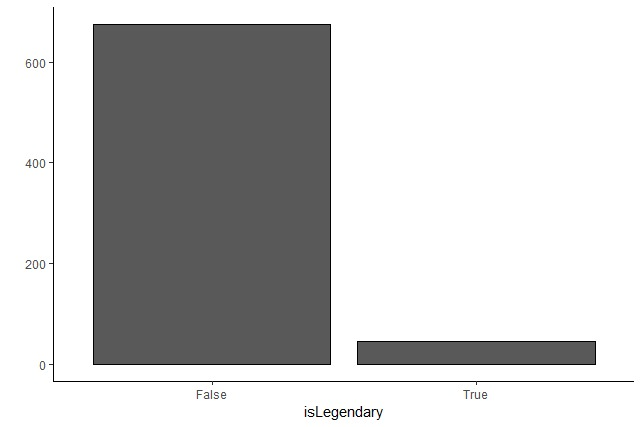
\includegraphics[width=80mm]{figures/barchart.png}}
\caption{\label{barplot:fig} Distribuzione dell'attributo ``$isLegendary$"}
\end{figure}


\subsubsection{Approccio Preliminare}
Con lo scopo di restringere la rosa di modelli per la classificazione, abbiamo inizialmente affrontato il problema testando $7$ classificatori di diversa natura:

$DecisionTree$, $J$-$48$ e $RandomForest$ tra gli euristici,

$Logistic$ e $SimpleLogistic$ tra i regression based, 

$NaiveBayes$ e $NBTree$ tra i probabilistici.

Al fine di eseguire la classificazione con algoritmi differenti tra loro, abbiamo deciso di selezionare i 4 classificatori che si sono rivelati i migliori tra quelli testati, scegliendoli in base al criterio dell’accuracy (vedasi Fig.~\ref{preliminar_leg:fig}) e dell'interpretabilità:

$J$-$48$, $RandomForest$

$SimpleLogistic$

$NBTree$\\
\begin{figure}
\frame{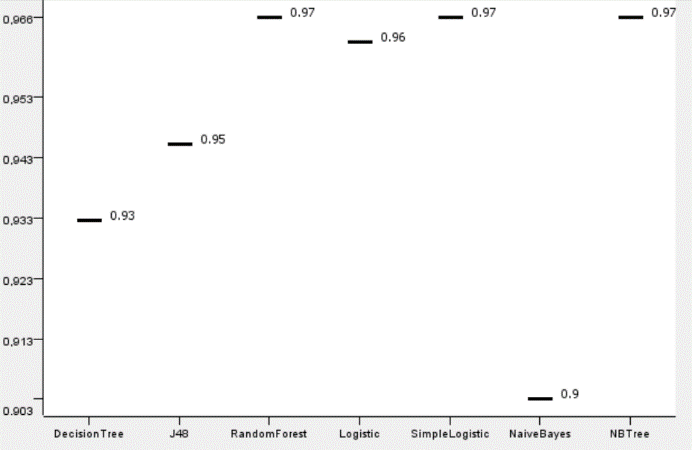
\includegraphics[trim={0, 0cm, 0, 0},width=85mm,angle=0,clip=]{figures/Preliminar_acc_leg.png}}
\caption{\label{preliminar_leg:fig} Confronto preliminare tra le accuracy di vari modelli di classificatori.}
\end{figure}
Notiamo anche che i valori di $F$-$measure$, riportati in Fig.~\ref{prelim_fmeas_leg:fig}, sono sistematicamente più bassi rispetto alle relative accuracy, ma ne seguono mediamente l'andamento: questo fatto non stupisce, in quanto l'attributo è estremamente sbilanciato nelle sue modalità e sul $test\ set$ non viene effettuato $oversampling$.

\begin{figure}
\frame{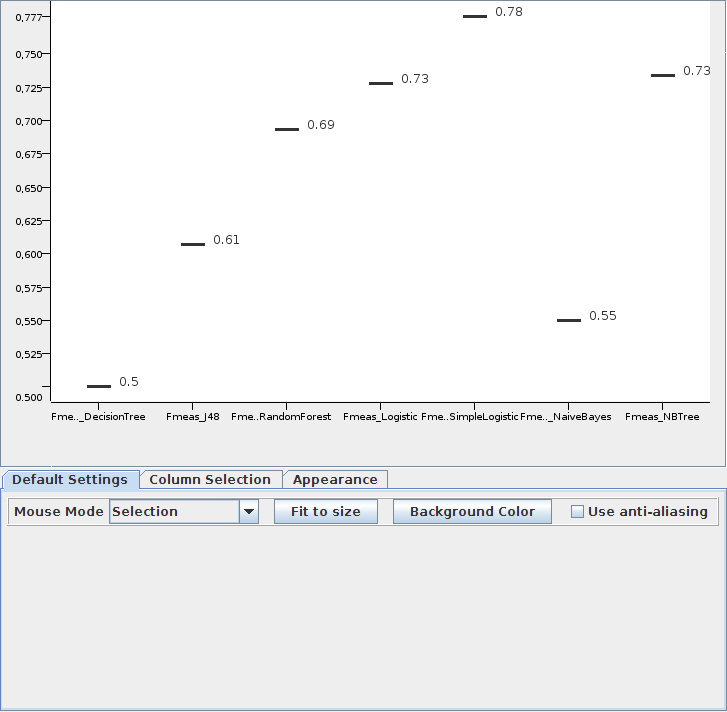
\includegraphics[trim={0, 9.8cm, 0, 0},width=85mm,angle=0,clip=]{figures/Preliminar_fmeas_leg.png}}
\caption{\label{prelim_fmeas_leg:fig} Performance preliminare: $F$-$measure$ relativa ai modelli di classificazione testati.}
\end{figure}


\subsection{Feature Selection}
Al fine di ottimizzare le prestazioni dei classificatori abbiamo deciso di selezionare le variabili rilevanti per ogni modello che ci appresteremo a utilizzare per eliminare, così, attributi ridondanti o irrilevanti. L'approccio da noi scelto è quello del “wrapper” per cui è il classificatore stesso ad essere utilizzato per trovare il subset ottimale tra gli attributi disponibili, attraverso il nodo KNIME AttributeSelectedClassifier. %(FIX: ADD ref/CIT). 
Il classificatore viene istruito con il validation set con lo scopo di determinare, per ogni modello, il sottoinsieme ottimale di attributi. Come effetto collaterale di questa procedura, essendo stato ricavato il subset ottimale di attributi per ogni modello dall'utilizzo di questa porzione di dati, da qui in avanti quest'ultima non verrà utilizzata laddove si sfrutti la conoscenza ottenuta.
In prima istanza esaminiamo i risultati della feature selection: per ogni classificatore sono stati scelti quasi sempre gli stessi attributi, segno che questi sembrerebbero essere piuttosto caratterizzanti rispetto agli altri. Per i vari modelli le feature selezionate sono:
\begin{itemize}


\item $J$-$48$: $Attack$, $Defense$, $Sp\_Atk$, $Sp\_Def$, $Speed$,
\\ $Height\_m$.
\\
\item $RandomForest$: $HP$, $Attack$, $Defense$, $Sp\_Atk$, $Sp\_Def$, $Speed$, $Height\_m$.

\item $SimpleLogistic$: $HP$, $Defense$, $Sp\_Atk$, $Sp\_Def$, $Speed$, $Height\_m$, $Weight\_kg$.

\item $NBTree$: $Defense$, $Sp\_Atk$, $Sp\_Def$, $Speed$, $Height\_m$, $Weight\_kg$.

\end{itemize}


\subsection{Classificazione}
Una volta selezionati gli attributi più appropriati per la classificazione abbiamo effettuato un confronto tra le performance dei diversi classificatori ottenute applicando la feature selection (utilizzando sia il metodo dell’$hold\ out$ che quello del $K$-$Folds\ Cross\ Validation$) e quelle ottenute sfruttando tutti gli attributi.

Come riportato in Fig.~\ref{holdout_acc_leg:fig},
\begin{figure}
\frame{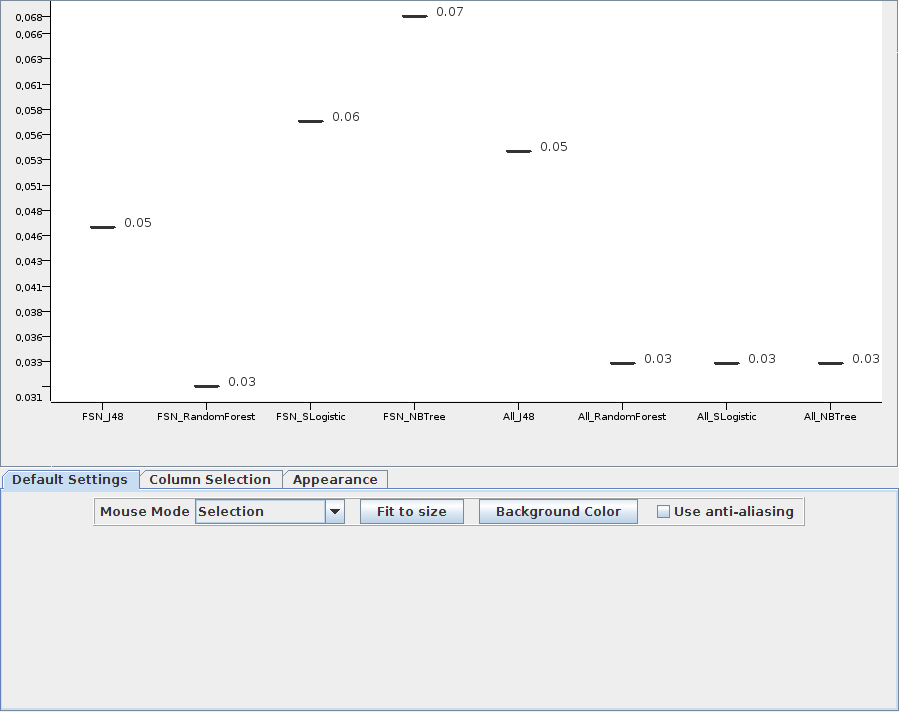
\includegraphics[trim={0, 9.8cm, 0, 0},width=85mm,angle=0,clip=]{figures/holdout_acc_leg.png}}
\caption{\label{holdout_acc_leg:fig} Errore ($1-acc$) relativo ai modelli di classificazione adottati.}
\end{figure}
i risultati sono tra loro molto simili, anche considerando il fatto che la feature selection ha mediamente rimosso 1 o 2 attributi da quelli disponibili. 
L'utilizzo della $K$-$Folds\ Cross\ Validation$ non  mostra differenze significative rispetto alla stima con l’$holdout$. 
L'elemento più significativo risultante da questa analisi (implementando la $Feature\ Selection$) lo si ottiene osservando gli intervalli di confidenza relativi all'accuracy dei modelli adottati: nello specifico si può apprezzare un  calo di prestazioni del $SimpleLogistic$ e del $NBTree$ in favore degli algoritmi $J$-$48$
e $RandomForest$, come riporta la Fig.~\ref{acc_leg:fig}. 
\begin{figure}
\frame{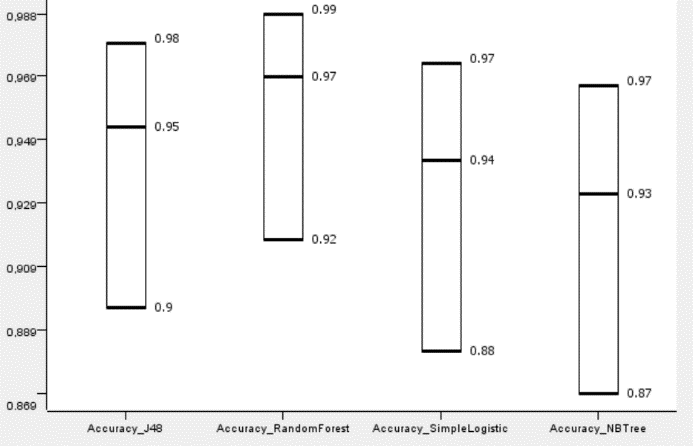
\includegraphics[trim={0, 0cm, 0, 0},width=85mm,angle=0,clip=]{figures/acc_leg.png}}
\caption{\label{acc_leg:fig} Intervallo di confidenza per l'accuracy relativo ai modelli di classificazione adottati (ottenuti con semplice $hold\ out$). L'intervallo in questione è ricavato con soglia di confidenza $1-\alpha=0.99$.}
\end{figure}

Questo trend non si limita solo alla stima dell'accuratezza ma anche alla misura della $F$-$measure$; come mostrato in Fig.~\ref{fmeas_leg:fig}, in generale i classificatori regression based e probabilistici sembrano soffrire maggiormente la riduzione degli attributi disponibili rispetto ai classificatori euristici.
\begin{figure}
\frame{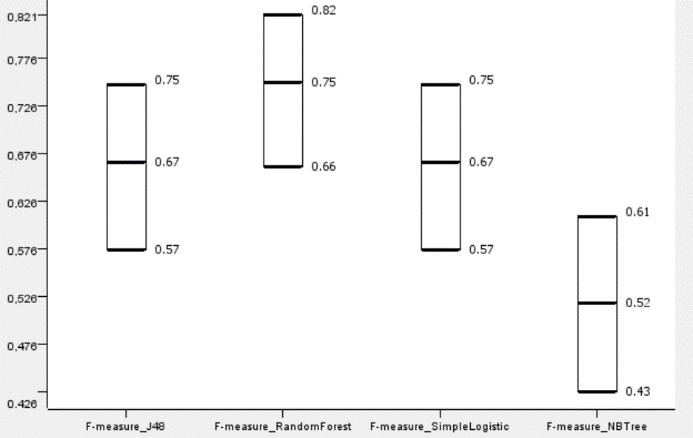
\includegraphics[trim={0, 0cm, 0, 0},width=85mm,angle=0,clip=]{figures/fmeas_leg.png}}
\caption{\label{fmeas_leg:fig} Come in Fig.~\ref{holdout_acc_leg:fig} ma per le misure di $F$-$Measure$.}
\end{figure}

\subsection{\textit{ROC Curves}}
Per ultimo abbiamo esaminato l'andamento dei classificatori tramite le $ROC\ curves$ per avere un confronto tra le diverse probabilità di corretta classificazione degli eventi (isLegendary = True) al variare dell'errata classificazione dei non-eventi (isLegendary = False). La $ROC\ curve$ infatti rappresenta sull'asse delle ordinate il numero dei record positivi di un certo subset dei dati espresso come percentuale del numero totale dei record positivi, mentre sull'asse delle ascisse il numero di record negativi del subset come percentuale di tutti i record negativi. Tra i modelli testati, il modello con la probabilità più alta di identificare bene i Pokémon ``leggendari", basandoci sull'area sottostante la $ROC\ curve$ riportata in Tab.~\ref{Roc_leg:tab}, è il $SimpleLogistic$, mentre facendo riferimento esclusivamente ai valori raggiunti da misure di performance come accuratezza ed $F$-$measure$ il migliore sembrerebbe essere il $RandomForest$. Tuttavia, osservando le stime degli intervalli di confidenza, la differenza tra i modelli non risulterebbe significativa.

\begin{table}
\begin{center}
\begin {tabular}{c | c }
\hline
\hline
P(isLegendary=True) & area sotto la curva\\
\hline
 $J$-$48$ & 0,9299\\
$RandomForest$& 0,8943\\
$SimpleLogistic$&0,9823\\
$NBTree$&0,8568\\
\hline
\hline
\end{tabular}
\end{center}
\caption{\label{Roc_leg:tab}
Area sottesa alle $ROC\ curves$ per $isLegendary=True$.}
\end{table}
\newpage
\section{Classificazione di ``$rarity\_class$”}
\subsection{Preprocessing}
Per la classificazione di ``$rarity\_class$”, che si pone l'obiettivo di individuare quali aspetti concorrano a determinare la difficoltà di cattura di un Pokémon, escludiamo a priori 4 attributi dei 22 iniziali:

$Body\_Style$, $Color$, $Name$: poiché non hanno alcuna utilità per la classificazione.

$Catch\_Rate$, essendo la feature dalla quale è stata ricavata la variabile obiettivo ``$rarity\_class$”.

\subsubsection{Discretizzazione}
Nel videogioco in questione, quando un allenatore incontra un Pokémon selvatico interessante (ad esempio piuttosto raro, o piuttosto forte dal punto di vista delle statistiche), il giocatore può tentare di catturarlo: l'esito di tale processo è sempre incerto, e tale ``suspense" è caratteristica di questa fase del gioco. L'esito di questo processo di cattura è influenzato da due fattori: in primo luogo dal Pokémon in questione (l'informazione della facilità o meno di cattura di uno specifico Pokémon è appunto codificata nella variabile $Catch\_Rate$), mentre il secondo fattore avente un ruolo importante nella fase di cattura è un moltiplicatore random, che rende più casuale e quindi incerto il risultato, aumentando il divertimento (nonché gli scherzosi sfoghi d'ira da parte del giocatore, qualora il tanto desiderato Pokémon fugga evitando la cattura). 
Con lo scopo di svolgere un lavoro di classificazione riguardante $Catch\_Rate$ ma non volendosi rivolgere alla variabile codificata così come presente nel dataset, si è proceduto alla sua discretizzazione codificando una nuova variabile denominata “$rarity\_class$”, categorica, con lo scopo di catalogare ogni Pokémon in una delle tre classi: “Common”, “Uncommon”, “Rare”.
Stante quanto riportato sopra, questo processo di discretizzazione ha anche lo scopo di rendere più verosimile l'informazione ottenuta riguardo alla facilità di cattura di un Pokémon particolare: infatti, riducendo la variabilità iniziale di $Catch\_Rate$ (nonché la dimensionalità della stessa), si può considerare in un certo senso meno importante la randomicità del processo di cattura, giacché si ottiene una informazione meno predittiva nello specifico, ma "mediata" (più generale) e quindi più affidabile.
La discretizzazione è avvenuta basandosi sui quantili visualizzati osservando la particolare funzione di ripartizione della variabile $Catch\_Rate$, riportata in Fig.~\ref{ripartiz:fig}.
\begin{figure}
\frame{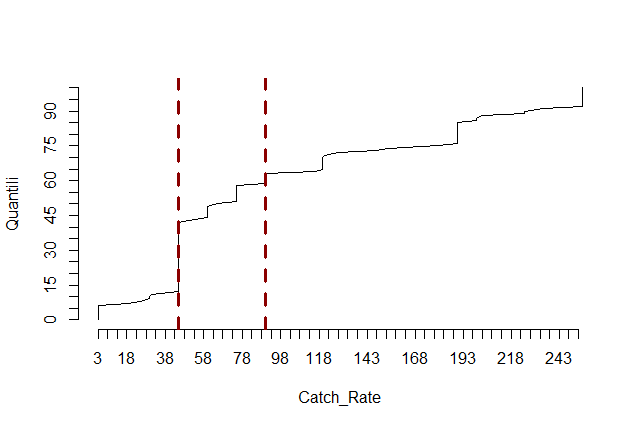
\includegraphics[trim={0, 0cm, 0, 0},width=85mm,angle=0,clip=]{figures/Rplot.png}}
\caption{\label{ripartiz:fig} Funzione di ripartizione della feature $Catch\_Rate$. Le linee verticali tratteggiate rappresentano la divisione in intervalli discreti associati ai valori della nuova variabile $rarity\_class$.}
\end{figure}
 Eseguendo dei binning manuali, abbiamo cercato di rispettare un criterio di “rarità”:
\begin{itemize}
\item per la classe “Rare” sono stati scelti i Pokémon con valore di $Catch\_Rate < 45$, ovvero circa l'$11\%$ del dataset; 
\item per “Uncommon” sono stati selezionati quelli aventi valore di $45 \leq Catch\_Rate < 90$ così da selezionare il successivo $47\%$; 
\item per i “Common” sono stati selezionati tutti quelli con $Catch\_Rate \geq 90$, comprendendo così il rimanente $42\%$ dei record.
\end{itemize} 
 Vale la pena di notare che la nuova variabile così ottenuta è stata utilizzata solo per questa seconda classificazione.
\subsubsection{Missing Replacement}\label{missing:sec}
Una volta effettuato il $preprocessing$, procediamo all'imputazione dei dati mancanti presenti nelle variabili $Type\_2$, $Pr\_Male$ e $Egg\_Group\_2$. Avendo una conoscenza del dominio si è deciso di procedere per imputazione manuale laddove vi sia la presenza di missing value, trattandosi di poche osservazioni. Per i Pokémon sprovvisti di $Type\_2$, dato che sono molti, si è creata una nuova classe denominata “NoOne” proprio perché il fatto stesso che un Pokémon non possieda un secondo tipo rappresenta di per sé un'informazione. In modo analogo si è proceduto per $Egg\_Group\_2$. Per $Pr\_Male$, in corrispondenza dei Pokémon per cui non era specificato il sesso, ovvero per quelli con hasGender uguale a “false” ci si è limitati ad inserire $Pr\_Male=0$, poiché non vi è alcuna possibilità di rintracciarli in versione maschile se questi ultimi non possiedono una distinzione sessuale.

%Lo stesso procedimento eseguito nella sezione \ref{missing:sec} (FIX: insert previous missing replacement section) viene iterato qui.

\subsubsection{Approccio Preliminare}
Una prima fase di approccio alla classificazione consiste in una valutazione del comportamento di diversi classificatori, che abbiamo testato in modo preliminare utilizzando tutti i records (divisi tra training e test set seguendo la consueta proporzione del $67\%$ e $33\%$).
\begin{figure}

\frame{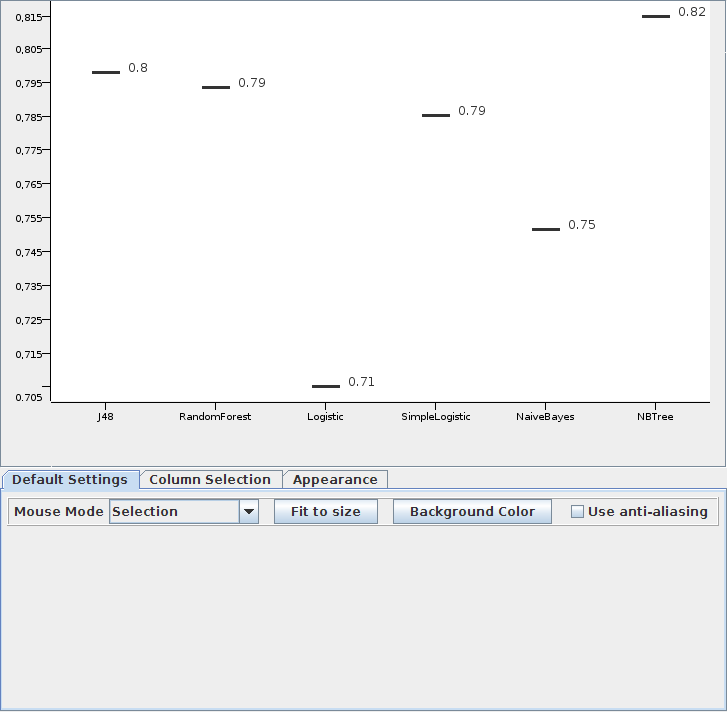
\includegraphics[trim={0, 9cm, 0, 0},width=85mm,angle=0,clip=]{Preliminar_acc.png}}
\caption{\label{preliminar:fig} Confronto preliminare tra le accuracy di vari modelli di classificazione inizialmente testati.}
\end{figure}

Abbiamo quindi selezionato quattro modelli di classificazione, scelti in base alle migliori performance iniziali, riportate in Fig.~\ref{preliminar:fig}: \textbf{$J$-$48$}, \textbf{$RandomForest$}, \textbf{$SimpleLogistic$}, \textbf{$NBTree$}. In particolare, a un primo approccio tali classificatori sembrano equivalentemente performanti: ci proponiamo quindi di investigare ulteriormente, con metodi di apprendimento più sofisticati e affidabili, per tentare  di stabilire se uno dei quattro modelli possa risultare migliore degli altri.

\newpage
\subsection{Feature Selection}
Partizioniamo inizialmente il dataset estraendo tramite un campionamento stratificato (rispetto a $rarity\_class$) un $Validation$ $Set$ composto dal $15\%$ dei records.
Utilizzando questo sottoinsieme, procediamo quindi con la $Feature\ Selection$, sfruttando dei wrappers che restituiscono per ciascun classificatore le seguenti variabili valutate più rilevanti:
\begin{itemize}
\item \textbf{$J$-$48$}: $Total$, $hasGender$, $Pr\_Male$, $hasMegaEvolution$;
\item \textbf{$RandomForest$}: $Total$, $HP$, $Sp\_Atk$, $hasGender$, 

$Pr\_Male$, $hasMegaEvolution$, $Height\_m$;
\item \textbf{$SimpleLogistic$}: $Total$, $Defense$, $Sp\_Atk$, $Pr\_Male$;
\item \textbf{$NBTree$}: $Type\_2$ $Total$, $Pr\_Male$, $Egg\_Group\_1$,
 
 $hasMegaEvolution$.
\end{itemize}

Possiamo notare come alcuni attributi vengano selezionati in tutti i classificatori: in particolare, risultano comunemente rilevanti $Total$, come da aspettative essendo una variabile riassuntiva delle statistiche di ciascun Pokémon, e dunque molto descrittiva, e $Pr\_Male$. La selezione di quest'ultimo attributo si spiega considerando che i Pokémon Leggendari, ovvero molti tra i più rari, non hanno un genere definito, per cui per costoro la probabilità di avere sesso maschile risulta caratteristicamente $Pr\_Male=0$, come accennato nella Sez.~\ref{missing:sec}. 

In seguito compareremo le performance ottenute utilizzando questi attributi selezionati con quelle ricavate sfruttando tutte le feature disponibili.

\subsection{Classificazione}

Partizioniamo ulteriormente (sempre con $stratified\ sampling$) i restanti records (scartando quindi il $validation$ $set$ usato per la $Feature\ Selection$) in un $training$ $set$ ($67\%$ dei records) e un $test$ $set$ ($33\%$).
Procediamo quindi con l'addestramento dei classificatori, utilizzando sostanzialmente l'approccio della $K$-$FOLDS$ $Cross\ Validation$ con $k=10$ iterazioni. Come misure di performance abbiamo analizzato l'errore risultante dalla classificazione (inteso come $1-acc$ in $\%$) e la $F-Measure$, poiché il $test$ $set$ risultante dalle partizioni è composto da pochi records e la classe $Rare$ risulta leggermente sbilanciata.
Otteniamo le performance riportate in Fig.~\ref{error:fig}. %\ref{fmeas:fig}.
\begin{figure}
\frame{\includegraphics[trim={0, 9cm, 0, 0},width=80mm,angle=0,clip=]{figures/error.png}}
\caption{ \label{error:fig} Performance: errore ($1-acc $) per ogni classificatore, dopo l'apprendimento tramite $Cross\ Validation$.
Si possono confrontare i risultati ottenuti con (voci con prefisso $FS$) e senza (voci con prefisso $All$) Feature Selection.}
\end{figure}

\begin{figure}
%\includegraphics[width=80mm]{Images/error.png}
\frame{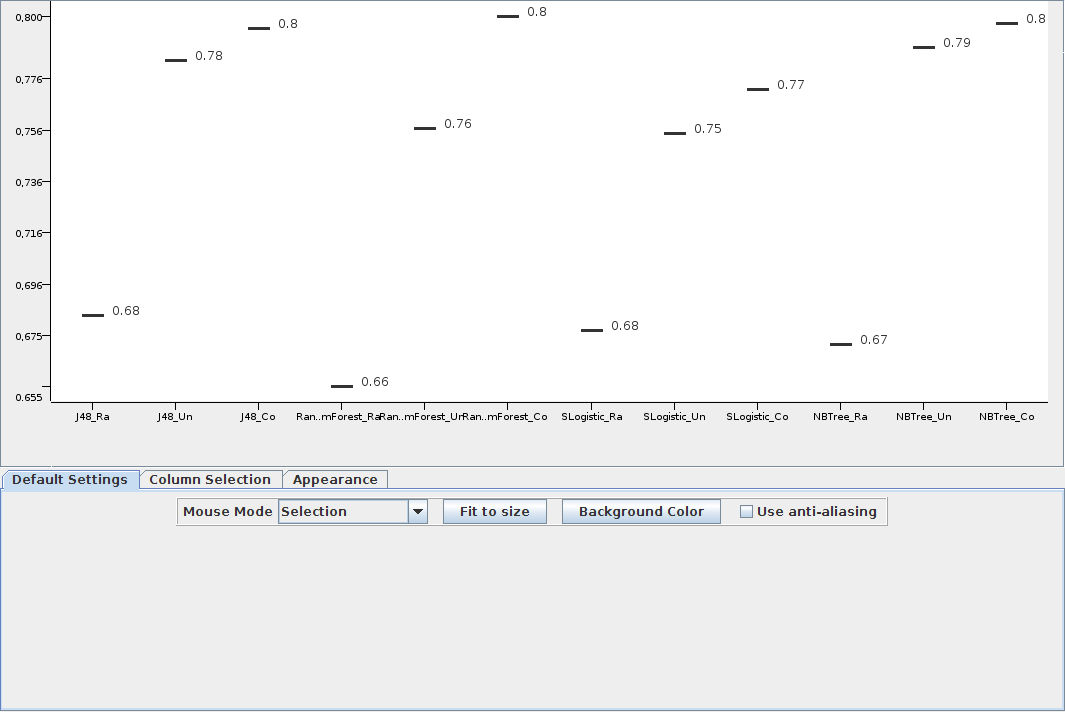
\includegraphics[trim={0, 9cm, 0, 0},width=80mm,angle=0,clip=]{figures/fmeas.png}}
\caption{ \label{fmeas:fig} Performance: $F$-$measure$ per ogni classificatore, dopo l'apprendimento tramite $Cross\ Validation$.}
\end{figure}
Possiamo notare che le performance relative alla classificazione dei records appartenenti alla classe $Rare$ sono sistematicamente peggiori rispetto a quelle relative alle altre classi: questo risultato è spiegato con lo sbilanciamento del dataset relativamente a questa classe, che risulta leggermente sottorappresentata, fatto che provoca un peggior apprendimento del classificatore.
Nonostante ciò, per tutti e quattro i classificatori le performance sono paragonabili: in prima analisi non si distingue un classificatore nettamente migliore degli altri.
Per approfondire ulteriormente la comparazione tra classificatori, riportiamo in Fig.~\ref{confidence:fig} un'analisi dei $confidence \ interval$ relativamente all'accuracy dei modelli \cite{tan}.
Notiamo che la performance media dei classificatori si assesta in tutti i casi intorno a $acc_{mean}\approx 0.8$, e possiamo notare un leggero ma generale aumento delle performance laddove sia stata applicata la $Feature\ Selection$, segno che la riduzione della complessità del sistema non ha portato a una perdita di informazione, ma ha anzi permesso di mantenere performance simili (addirittura leggermente migliori) e di ottenere un risultato decisamente più interpretabile.

%FIX: produrre eventualmente grafico F-measure
\begin{figure}
\frame{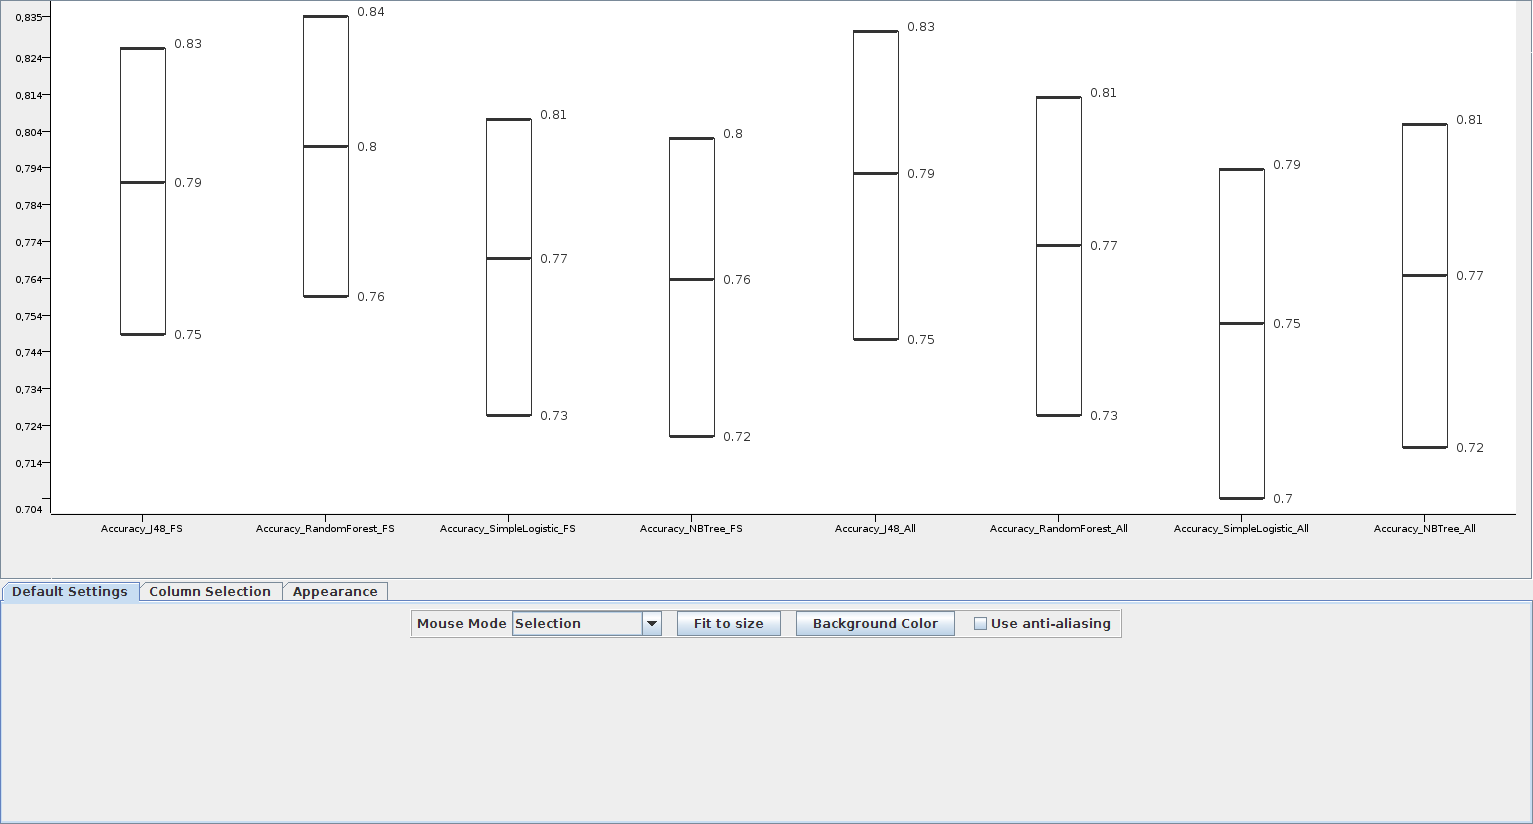
\includegraphics[trim={0, 9cm, 0, 0},width=80mm,angle=0,clip=]{figures/confidence_CrossValid.png}}
\caption{ \label{confidence:fig} Confronto dei confidence interval (accuracy) per ogni classificatore, sia nel caso di $Feature Selection$ (FS) sia nel caso di inclusione di tutti gli attributi (All). Si può notare che gli intervalli di confidenza si sovrappongono reciprocamente, segno che i risultati dei vari classificatori sono compatibili, e i modelli stessi risultano equivalenti per questo tipo di problema.
L'apprendimento avviene tramite $Cross$ $Validation$.}
\end{figure}

%\begin{figure}
%\includegraphics[trim={0, 9cm, 0, 0},width=80mm,angle=0,clip=]{figures/confmeas.png}
%\caption{ \label{confmeas:fig} Confronto dei confidence interval ($F$-$Measure$) per ogni classificatore. Si può notare che gli intervalli di confidenza si sovrappongono reciprocamente, segno che i risultati dei vari classificatori sono compatibili, e i modelli stessi risultano equivalenti per questo tipo di problema.}
%\end{figure}
\newpage
\subsection{\textit{ROC Curves}}
Analizzando le $ROC\ Curves$, si osserva una differenza piuttosto significativa tra le aree sottese alle $ROC\ Curves$ corrispondenti alle diverse modalità di $rarity\_class$, come mostrato in Tab.~\ref{Roc_rarity:tab}.
Sembrerebbe infatti che la classe $Uncommon$ risulti di più difficile classificazione per via della sua posizione intermedia tra i due intervalli estremi $Common$ e $Rare$. Infatti, questi ultimi sono meglio caratterizzati proprio a causa della loro natura estremale. 
Emergono quindi i limiti di una discretizzazione non supervisionata ma effettuata manualmente, seppur guidata da osservazioni qualitative (come riportato in Fig.~\ref{ripartiz:fig}).
%Of course cite Tab.~\ref{Roc_rarity:tab}
\begin{table}
\begin{center}
\begin {tabular}{c | c | c |c}
\hline
\hline
Classificatore & $P(Uncommon)$&$P(Common)$ & $P(Rare)$\\
\hline
$J$-$48$ &0.855& 0.903 &0.843\\
$RandomForest$& 0.874& 0.908&0.920\\
$SimpleLogistic$&0.825& 0.896& 0.891\\
$NBTree$&0.856& 0.896& 0.890\\
\hline
\hline
\end{tabular}
\end{center}
\caption{\label{Roc_rarity:tab}
Area sottesa alle $ROC\ curves$ per ogni modalità di $rarity\_class$.}
\end{table}

%\section{Clustering}
%Ci siamo poi ulteriormente domandati se esistessero delle ``famiglie" ben determinate di Pokémon, ovvero se questi fossero in qualche modo distinguibili e raggruppabili in diversi sottoinsiemi in base alle loro statistiche. Abbiamo dunque applicato degli algoritmi di clusterizzazione al nostro dataset (dopo aver implementato il $missing$ $replacement$ come descritto in Sez.~\ref{missing:sec}). In particolare, abbiamo testato i seguenti modelli:
%\begin{itemize}
%\item il classico $k$-$means$ e il $fuzzy\ c-means$  per quanto riguarda i (FIXMEH)
%\item $Hierarchical Clustering$ (Weka)
%\item $SOM$
%\end{itemize}

%FIX: bisogna giustificare, oltre che con grafici nei quali non è visibile presenza di clusters, anche con il calcolo di qualche coefficente , in modo da avere un risultato quantitativo.


%I risultati del clustering non sono stati particolarmente positivi, ovvero nessun algoritmo è riuscito a individuare dei sottoinsiemi internamente coerenti e separati rispetto al resto del dataset: del resto il risultato non è inaspettato, in quanto in qualità di esperti del settore, sappiamo bene che ogni specie di Pokémon, pur condividendo alcune caratteristiche con altri, è creato in modo da essere unico e avere un caratteristico mix di statistiche, diverso da tutti gli altri.
%Di fatto la cluster analisys conferma l'intuizione dell'impossibilità di categorizzare i Pokémon in ``classi" distinte e ben separate, data l'intrinseca diversità volutamente implementata dai loro creatori.

\section{Conclusioni}
In conclusione riportiamo sinteticamente le risposte alle principali domande di ricerca.
\begin{itemize}
\item \`E possibile individuare i Pokémon leggendari solamente in base alle loro statistiche ``fisiche"? 

La risposta è sì, e con risultati piuttosto consistenti: infatti, l'accuracy (nonché la misura di $F$-$Measure$) raggiunta dai classificatori per tale compito è piuttosto alta, e tutti i modelli di classificazione usati per l'analisi si sono rilevati sostanzialmente equivalenti e ben performanti.
In particolare abbiamo scoperto che bastano pochi attributi comuni selezionati attraverso $Feature$ $Selection$ per ottenere ottimi risultati di classificazione, segno che il risultato è chiaramente interpretabile tramite il significato che questi attributi assumono nel mondo dei Pokémon.
In linea di massima possiamo affermare che i Pokémon etichettati -dai creatori del gioco- come leggendari non posseggono tale titolo solo per ragioni di trama o convenienza, ma perché dotati a tutti gli effetti di statistiche di combattimento generalmente piuttosto elevate.

\item \`E possibile predire in base alle statistiche generali la facilità di cattura di un Pokémon?

La risposta è (parzialmente) sì: con la classificazione multibinaria che abbiamo effettuato, avente come target la variabile $rarity\_class$ da noi creata, abbiamo ottenuto un'accuracy media dell'ordine di $acc_{mean}\approx 0.8$, comune a tutti i classificatori adottati. Tale risultato indica che i relativamente pochi attributi selezionati (dalla $Feature$ $Selection$) influenzano in modo significativo il processo di cattura.

I risultati sono probabilmente incrementabili applicando direttamente una regressione alla variabile continua $catch\_rate$, come eseguito ad esempio in \cite{report}, tuttavia la risposta alla domanda principale sarebbe in questo frangente offuscata (se non contraddetta, in alcuni casi) dal peso del fattore random che gioca un ruolo importante durante il processo di cattura. Con la nostra discretizzazione pensiamo di ottenere un risultato più affidabile in termini di riscontro nel gioco, benché meno predittivo nello specifico.

%\item \`E possibile individuare delle famiglie distinte e ben separate di Pokémon? 

%L'esito del processo di clusterizzazione applicato suggerisce che basandoci sulle statistiche dei Pokémon non emerge una chiara struttura di cluster all'interno del mondo dei Pokémon, probabilmente per via della diversità intrinseca di ciascun esemplare.
\end{itemize}

%------------------------------------------------------------------
%  BIBLIOGRAPHY
%------------------------------------------------------------------

%\section*{References}
\vspace*{6cm} %FIX
\begin{thebibliography}{9}
 \bibitem {pokemon}
\url{https://www.kaggle.com/alopez247/pokemon}

\bibitem{brownlee}
 Brownlee J. 8 tactics to combat imbalanced classes
in your machine learning dataset. \url{https://machinelearningmastery.com}, 2015.

\bibitem{tan}
Tan P.-N. Steinbach M. Kumar V. Introduction to data
mining. \url{http://www.uokufa.edu.iq/staff/ehsanali/Tan.pdf},  2006.

\bibitem{report}
Statistical analysis of Pokémon, Asier López Zorrilla, \url{https://www.kaggle.com/alopez247/pokemon}, 2017.
\end{thebibliography}
 \end{document}
